
\documentclass[10pt]{article}
\usepackage{microtype}
\usepackage{graphicx} % Required for inserting images
\usepackage{blindtext}
\usepackage{geometry}
\usepackage{multirow}
\usepackage{enumerate}
\usepackage{tabto}
\usepackage{inputenc}
\usepackage{enumitem,amssymb}
\newlist{todolist}{itemize}{2}
\setlist[todolist]{label=$\square$}
 \geometry{
 a4paper,
 total={170mm,257mm},
 left=20mm,
 top=10mm,
 }
\begin{document}
\begin{flushright}JEE (Advanced) 2022 \;\;\;\;\;\;\;\;\;\;\;\;\;\;\;\;\;\;\;\;\;\;\;\;\;\;\;\;\;\;\;\;\;\;\;\;\;\;\;\;\;\;\;\;\;\;\;\;\;\;\;\;\;\;\;\;\;\;\;\;\;\;\;\;\;\;\;\;\;\;\;\;\;\;\;\;\;\;\;\;\;\;\;\;\;\;\;\;\;\;\;\;\;\;\;\;\;\;\;\;\;\;\;\;\;\;\;\;\;\;\;Mohan Manjhi\end{flushright}
$$\textbf{------------------------------------------------------------------------------------------------------------------------------}$$
\begin{center}
\fbox{\parbox{6.5in}{
\begin{center}
    
\includegraphics[width=0.25\linewidth]{iitB.png}
\end{center} 
\hspace*{4ex}Name : Mohan Manjhi \tab  \hspace*{10ex}Max Marks : 70\\ \\ \hspace*{4ex}Branch : C.S.E \tab  \hspace*{10ex}Min Marks : 22\\ \\ \hspace*{4ex}Subject : Latex Assignment\tab  \hspace*{10ex}Time : 03:00 HRS  \\ \\
\hspace*{4ex}Signature of the Examiner with date \tab \hspace*{10ex}Signature of the Scrutinizer with date\\ \\
\hspace*{4ex}------------------------------------------------\tab \hspace*{12ex}------------------------------------------------\\ \\
}}

\end{center}
READ THE INSTRUCTIONS CAREFULLY \\
GENERAL \\
\begin{itemize}
    \item This sealed booklet is your Question Paper. Do not break the seal till you are told to do so.
\end{itemize}

\begin{itemize}
    \item Immediately after breaking the seal of the booklet, verify that the booklet contains 23 pages and that all the 16 questions along with the options are legible.
\end{itemize}
\begin{itemize}
    \item Report immediately about any missing or torn sheet in this booklet and ask for a replacement of the booklet from the invigilator. No replacement will be allowed after 15 minutes of the starting of the examination.
\end{itemize}
\begin{itemize}
    \item Write your Name, Roll Number, JEE (Advanced) 2022 Rank and other details in the space provided and nowhere else. No distinctive / identification mark of any type is to be put anywhere else in this booklet.
\end{itemize}
\begin{itemize}
    \item Answers are to be written only in the booklet and within the space provided beside / below each Question and nowhere else. Answers written in nondesignated place will not be evaluated. 
\end{itemize}
\begin{itemize}
    \item Blank spaces are provided within this booklet for rough work.
\end{itemize}
\begin{itemize}
    \item Do not deface this booklet or detach or mutilate any sheet from the booklet. Such acts lead to disqualification.
\end{itemize}

\begin{itemize}
    \item All the questions are compulsory.
\end{itemize}

\newpage
\begin{flushright}JEE (Advanced) 2022 \;\;\;\;\;\;\;\;\;\;\;\;\;\;\;\;\;\;\;\;\;\;\;\;\;\;\;\;\;\;\;\;\;\;\;\;\;\;\;\;\;\;\;\;\;\;\;\;\;\;\;\;\;\;\;\;\;\;\;\;\;\;\;\;\;\;\;\;\;\;\;\;\;\;\;\;\;\;\;\;\;\;\;\;\;\;\;\;\;\;\;\;\;\;\;\;\;\;\;\;\;\;\;\;\;\;\;\;\;\;\;Mohan Manjhi\end{flushright}
$$\textbf{------------------------------------------------------------------------------------------------------------------------------}$$
\begin{center}
\fbox{\parbox{6.5in}{\centering
\textbf{SECTION A: Architectural Awareness (Maximum Marks: 60)}\\
This section contains \textbf{FOUR} questions. Question 1 carries \textbf{30 marks}, Questions 2, 3 \\
and 4 carry \textbf{10 marks} each. There is \textbf{NO} negative marking}}
\end{center}
%\begin{center}\textbf{SECTION A: Architectural Awareness (Maximum Marks: 60)}
% \\
%This section contains FOUR questions. Question 1 carries %30 marks, Questions 2, 3 \\
%and 4 carry 10 marks each. There is NO negative marking.
%\end{center}
Q.1. This section contains \textbf{15 multiple choice questions}. Each question has four options, out of which
ONLY \\
\hspace*{5ex}ONE is correct. Mark the correct option with a tick
 \\ \begin{flushright}
    \textbf{(5 x 2 = 10 Marks)} 
\end{flushright}
(i) Which of the following bridges is laid over a sea? \\ \\
\hspace*{4ex}A. Godavari Bridge, Andhra Pradesh \\ \\
\hspace*{4ex}B. Pamban Bridge, Tamilnadu \\ \\
\hspace*{4ex}C. Howrah Bridge, West Bengal \\ \\
\hspace*{4ex}D. Mahatma Gandhi Setu, Bihar \\ 
%
\\ \\
(ii) In 2021, --------------------annual festivity got inscribed on the representative list of
Intangible Cultural \\
\hspace*{4ex}Heritage of Humanity by UNESCO. 
\\
%
\\
\hspace*{4ex}A. Makara Sankranthi \tab B. Ganesh Chaturthi \\ \\ \\
\hspace*{4ex}C. Durga Puja \tab D.Chhath Puja 
\\ \\
%
\\
(iii) Statue of which famous personality is called ‘Statue of Unity’? 
 \\ 
\\
%
\\
\hspace*{4ex}A. Mahatma Gandhi  \tab B. Dr. B. R. Ambedkar  
 \\ \\ \\
\hspace*{4ex}C. Sardar Vallabhbhai Patel   \tab D.Indira Gandhi 
\\ \\
%
\\
(iv) Which of the following historic gateways is sharing an edge with a water body? \\ 
\\
%
\\
\hspace*{4ex}A. Charminar, Hyderabad \tab B. India Gate, New Delhi \\ \\ \\
\hspace*{4ex}C. Rumi Darwaza, Lucknow  \tab D.Gateway of India, Mumbai 
\\ \\
%
\\ \\
(v) Which architect has designed the building ‘Church of Light’, located in Japan? 
 \\ 
\\
%
\\
\hspace*{4ex}A. Moshe Safdie \tab B. Fumihiko Maki 
 \\ \\ \\
\hspace*{4ex}C. Zaha Hadid   \tab D.Tadao Ando 
\\ \\
$$\textbf{------------------------------------------------------------------------------------------------------------------------------}$$
%
\begin{flushright}JEE (Advanced) 2022 \;\;\;\;\;\;\;\;\;\;\;\;\;\;\;\;\;\;\;\;\;\;\;\;\;\;\;\;\;\;\;\;\;\;\;\;\;\;\;\;\;\;\;\;\;\;\;\;\;\;\;\;\;\;\;\;\;\;\;\;\;\;\;\;\;\;\;\;\;\;\;\;\;\;\;\;\;\;\;\;\;\;\;\;\;\;\;\;\;\;\;\;\;\;\;\;\;\;\;\;\;\;\;\;\;\;\;\;\;\;\;Mohan Manjhi\end{flushright}
$$\textbf{------------------------------------------------------------------------------------------------------------------------------}$$
Q.2 Match the famous architects in column I with their renowned projects in column II. \hspace{10ex}\textbf{( Mark : 05)}\\
%
\\ \\ 
\hspace*{4ex}\textbf{Column I} \tab \textbf{Column II } 
\\ \\
\hspace*{4ex}(A) Charles Correa \tab (P) IIM Bangalore 
 \\ \\
\hspace*{4ex}(B) B V Doshi    \tab (Q)  Capitol Complex, Chandigarh 
\\ \\
\hspace*{4ex}(C) Bimal Pate \tab (R) Central Vista, New Delhi 
 \\ \\
\hspace*{4ex}(D)  Raj Rewal   \tab (S) Dakshina Chitra, Chennai  
\\ \\
\hspace*{4ex}(E)  Le Corbusier \tab (T) Bharat Bhawan, Bhopal 
 \\ \\
\hspace*{4ex} \tab (U) Parliament Library, New Delhi
\\ \\
%
Q.3 Match the material in Column I with the craft in Column II. \hspace{28ex}\textbf{( Mark : 05)}\\
%
\\ \\ 
\hspace*{4ex}\textbf{Column I} \tab \textbf{Column II } 
\\ \\
\hspace*{4ex}(A) Stone  \tab (P) Origami 
 \\ \\
\hspace*{4ex}(B) Paper    \tab (Q) Embroidery 
\\ \\
\hspace*{4ex}(C) Glass \tab (R) Carving 
 \\ \\
\hspace*{4ex}(D) Fabric   \tab (S) Carpentry 
\\ \\
\hspace*{4ex}(E) Metal  \tab (T)  Etching 
 \\ \\
\hspace*{4ex} \tab (U)  Filigree \\ \\ \\ \\ \\ \\ \\ \\ \\ \\ \\ \\ \\ \\ \\ \\ \\ \\ \\ \\ \\ \\
$$\textbf{------------------------------------------------------------------------------------------------------------------------------}$$
\newpage

\begin{flushright}JEE (Advanced) 2022 \;\;\;\;\;\;\;\;\;\;\;\;\;\;\;\;\;\;\;\;\;\;\;\;\;\;\;\;\;\;\;\;\;\;\;\;\;\;\;\;\;\;\;\;\;\;\;\;\;\;\;\;\;\;\;\;\;\;\;\;\;\;\;\;\;\;\;\;\;\;\;\;\;\;\;\;\;\;\;\;\;\;\;\;\;\;\;\;\;\;\;\;\;\;\;\;\;\;\;\;\;\;\;\;\;\;\;\;\;\;\;Mohan Manjhi\end{flushright}
$$\textbf{------------------------------------------------------------------------------------------------------------------------------}$$
Q.4 Refer to the following sketch of St. James’ Church, Delhi. Match the numbers mentioned in Column I 

(highlighted in the sketch) with corresponding building elements in Column II.\hspace{10ex}\textbf{( Mark : 05)}
    

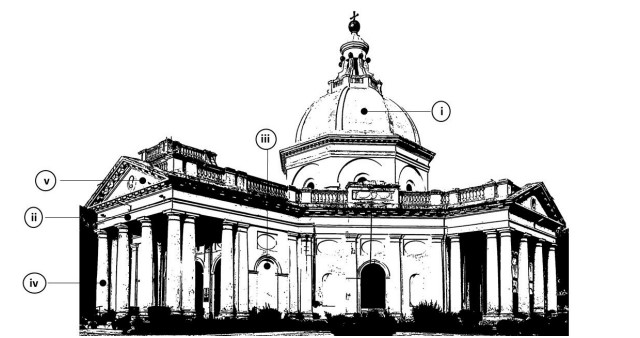
\includegraphics[width=1\linewidth]{q3.jpg}
\\ \\ \\ 
%
\\
\hspace*{4ex}\textbf{Column I} \tab \textbf{Column II} 
\\ \\
\hspace*{4ex}(A)  i   \tab (P) Column 
\\ \\
\hspace*{4ex}(B)  ii    \tab (Q) Pediment 
\\ \\
\hspace*{4ex}(C) iii \tab (R) Plinth 
\\ \\
\hspace*{4ex}(D) iv   \tab (S)  Dome 
\\ \\
\hspace*{4ex}(E) v  \tab (T)   Architrave 
\\ \\
\hspace*{4ex} \tab (U) Arch
 \\ \\ \\ \\ \\ \\ \\ \\ \\ \\ \\ \\ \\ \\ \\ \\
$$\textbf{------------------------------------------------------------------------------------------------------------------------------}$$
\nextpage
\begin{flushright}JEE (Advanced) 2022 \;\;\;\;\;\;\;\;\;\;\;\;\;\;\;\;\;\;\;\;\;\;\;\;\;\;\;\;\;\;\;\;\;\;\;\;\;\;\;\;\;\;\;\;\;\;\;\;\;\;\;\;\;\;\;\;\;\;\;\;\;\;\;\;\;\;\;\;\;\;\;\;\;\;\;\;\;\;\;\;\;\;\;\;\;\;\;\;\;\;\;\;\;\;\;\;\;\;\;\;\;\;\;\;\;\;\;\;\;\;\;Mohan Manjhi\end{flushright}
$$\textbf{------------------------------------------------------------------------------------------------------------------------------}$$
Q.5 Read the following statements and choose the correct options. \hspace{30ex}\textbf{( Mark : 07)}\\ \\
\hspace*{10ex}Statement A : Parapet is a type of window  \\
\hspace*{10ex}Statement B : Pile is a type of foundation
\\ \\
%
\hspace*{4ex}A. Both the statements A \& B are True \\ \\
\hspace*{4ex}B. Both the statements A \& B are False \\ \\
\hspace*{4ex}C. The statement A is True but statement B is False \\ \\
\hspace*{4ex}D. The statement B is False but statement A is True \\ 
%
\\
Q.6 Refer to the graphical representation of timber, shown in figure 1
 graphical representation shown in 
 
 figure 2, indicate? \tab \hspace{40ex}\textbf{( Mark : 07)}\\ \\
 %
 \\
\hspace*{10ex}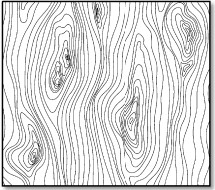
\includegraphics[width=0.40\linewidth]{q6_fig1.jpg}
\hspace*{4ex}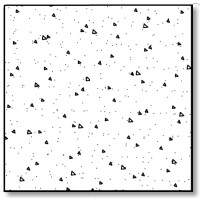
\includegraphics[width=0.36\linewidth]{q6_fig2.jpg} \\ \\
\hspace*{25ex} Figure 1 \tab \hspace*{15ex} Figure 2
 \\ 
\\
%
\\
\hspace*{4ex}A. Thermocol \tab B. Concrete 
 \\ \\ \\
\hspace*{4ex}C. Steel   \tab D.Brick 
\\ \\
Q.7   The least value of $ \alpha\epsilon R \hspace*{1ex}  for \hspace*{1ex} which \hspace*{1ex} 4\alpha x^2 + 1/x\ge 1, for \hspace*{1ex} all \hspace*{1ex} x>0, is $ \hspace{20ex}\textbf{( Mark : 07)} \\
\\
$\hspace*{4ex}A.\hspace*{4ex} \frac{1}{64} $\\ \\
$\hspace*{4ex}B.\hspace*{4ex} \frac{1}{32} $\\ \\
$\hspace*{4ex}C.\hspace*{4ex} \frac{1}{27} $\\ \\
$\hspace*{4ex}D.\hspace*{4ex} \frac{1}{25} $\\ 
\\ \\ \newpage 
\begin{flushright}JEE (Advanced) 2022 \;\;\;\;\;\;\;\;\;\;\;\;\;\;\;\;\;\;\;\;\;\;\;\;\;\;\;\;\;\;\;\;\;\;\;\;\;\;\;\;\;\;\;\;\;\;\;\;\;\;\;\;\;\;\;\;\;\;\;\;\;\;\;\;\;\;\;\;\;\;\;\;\;\;\;\;\;\;\;\;\;\;\;\;\;\;\;\;\;\;\;\;\;\;\;\;\;\;\;\;\;\;\;\;\;\;\;\;\;\;\;Mohan Manjhi\end{flushright}
$$\textbf{------------------------------------------------------------------------------------------------------------------------------}$$
Q.8 A system goes from A to B via two processes I and II as shown in figure. If $\Delta$U1 and $\Delta$U2 are the changes 

in internal energies in the processes I and II respectively, then \hspace{30ex}\textbf{( Mark : 07)}
\\
   $$ \centering
    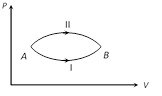
\includegraphics[width=0.25\linewidth]{Q8.jpg} $$
$\hspace*{4ex}A.\hspace*{4ex} \Delta U_{II} >\Delta U_I $\\ \\
$\hspace*{4ex}B.\hspace*{4ex} \Delta U_{II}<\Delta U_I $\\ \\
$\hspace*{4ex}C.\hspace*{4ex} \Delta U_I= \Delta U_{II} $\\ \\
\hspace*{4ex}D.\hspace*{4ex}  Relation between $\Delta$ $U_I$ and $\Delta$ $U_{II}$ can not be determined  \\ 
%
\\
Q.9 Consumers were polled about their favourite ice cream flavours in a survey. Draw a bar graph for 

the following data: \tab \hspace{42ex}\textbf{( Mark : 07)}\\
  \\   \begin{tabular}{|c|c|}
    \hline
        Flavour of Icecream & Frequency \\
    \hline
        Vanilla & 1\\
    \hline
        Strawberry & 5 \\
    \hline
        Chocolate & 12 \\
    \hline
        Mint Chocolate & 3 \\
    \hline
        Others & 6 \\
    \hline
    \end{tabular}  \\
\\ \\
Q.10 Examine the graph below carefully and answer the following questions. The graph depicts the results of a school’s students. \tab \hspace{42ex}\textbf{( Mark : 10)}

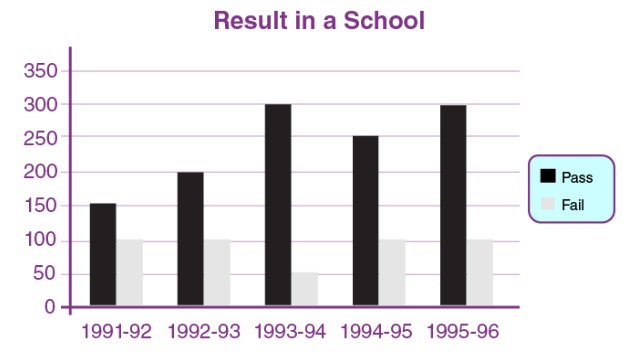
\includegraphics[width=0.85\linewidth]{q10.jpg} \\
%
\\
\hspace*{4ex}A. Which year has the smallest difference between the number of kids who passed and those who failed? \\ \\
\hspace*{4ex}B. In the last five years, what was the average number of kids who failed in school? \\ \\
\hspace*{4ex}C. How many times have the same number of kids failed? \\ \\

\end{document}